% Opciones empleadas:
%
%	a4paper -> indica el tama�o del papel, en este caso A4.
%	11pt -> tama�o de la fuente 11 puntos.
%	oneside -> s�lo escribimos en una cara del folio.
%
% Otras opciones interesantes:
%
%	twoside -> escribimos a doble cara.
%	openbib -> para que las referencias bibliogr�ficas tengan un salto de l�nea entre cada campo de la referencia.
%
\documentclass[a4paper,11pt,oneside]{book}

% codificaci�n latin1 y s�mbolos del idioma espa�ol (�, acentos, ...)
\usepackage[spanish]{babel}
\usepackage[latin1]{inputenc}

% puede que queramos usar el s�mbolo del euro.
\usepackage{eurosym}

% El paquete fancybox nos permite crear cajas de diferentes estilos con facilidad.
% http://www.ctan.org/get/macros/latex/contrib/fancybox/fancybox.pdf
% http://www.mackichan.com/index.html?techtalk/487.htm~mainFrame
\usepackage{fancybox}
\usepackage{multicol}
\usepackage{amsmath}

% Para incluir subfiguras.
\usepackage{subfigure}

% Para incluir gr�ficos en JPG => compilar con pdflatex.
\usepackage[pdftex]{graphicx}

% Para incluir gr�ficos EPS => compilar con latex.
%\usepackage[dvips]{graphicx}

% Para escribir en color...
%
% ... cuando compilamos con el comando ``latex''
%\usepackage[dvips,usenames]{color}
% ... uando compilamos con el comando ``pdflatex''
 \usepackage[pdftex,usenames,dvipsnames]{color}

% Espaciado y ajuste de m�rgenes
\usepackage{setspace}
\onehalfspacing
% \doublespacing
\setlength{\textwidth}{15cm}
\setlength{\textheight}{22cm}

% Paquete fancyhdr -> Para modificar la cabecera y pie de p�ginas.
% http://tug.ctan.org/tex-archive/macros/latex/contrib/fancyhdr/
\usepackage{fancyhdr}
\pagestyle{fancy}
\fancyhf{}
\fancyhf[HR]{\thepage}
\fancyhf[HL]{\nouppercase\rightmark}

% Package booktabs -> Para mejorar el aspecto de las tablas o cuadros.
% http://www.ctan.org/tex-archive/macros/latex/contrib/booktabs/
\usepackage{booktabs}

% Package rotating -> Para poder girar las tablas y dibujarlas a lo largo
% del folio en vez de a lo ancho.
\usepackage{rotating}

% Packages multicol y multirow, para manejar tablas de filas y columnas m�ltiples.
\usepackage{multicol}
\usepackage{multirow}

\usepackage{color}
\usepackage{xcolor}
\usepackage{caption}
\DeclareCaptionFont{white}{\color{white}}
\DeclareCaptionFormat{listing}{\colorbox{gray}{\parbox{\textwidth}{#1#2#3}}}
\captionsetup[lstlisting]{format=listing,labelfont=white,textfont=white}

 \usepackage{listings}
 \usepackage{courier}
 \lstset{
         basicstyle=\footnotesize\ttfamily, % Standardschrift
         numberstyle=\tiny,          % Stil der Zeilennummern
         numbersep=5pt,              % Abstand der Nummern zum Text
         tabsize=2,                  % Groesse von Tabs
         extendedchars=true,         %
         breaklines=true,            % Zeilen werden Umgebrochen
         keywordstyle=\textbf,
         frame=b,
         stringstyle=\textit, % Farbe der String
         showspaces=false,           % Leerzeichen anzeigen ?
         showtabs=false,             % Tabs anzeigen ?
         xleftmargin=17pt,
         framexleftmargin=17pt,
         framexrightmargin=5pt,
         framexbottommargin=4pt,
         %backgroundcolor=\color{lightgray},
         showstringspaces=false      % Leerzeichen in Strings anzeigen ?
 }

% Personalizamos la separaci�n entre p�rrafos...
\parskip=6pt

% Personalizamos el identado en la primera l�nea del nuevo p�rrafo...
\parindent=10pt

% Establecemos el n�mero m�ximo de niveles de profundidad en las secciones.
\setcounter{secnumdepth}{3}

% T�tulo
\title{GNOMECAT, un editor de ficheiros GNU Gettext para o proxecto GNOME}
% Autor
\author{Marcos Chavarr�a Teijeiro}
% Fecha
\date{\today}


\begin{document}

	% \maketitle sirve para generar autom�tica una portada predefinida, pero para un proyecto fin de carrera
	%	de FIC no sirvir�a porque no cumple las normas de presentaci�n. Podemos hacer dos cosas:
	% 1. Usarla e ignorar las normas (y asumir las consecuencias que pueda tener)
	% 2. Hacernos una portada en LaTeX que cumpla las normas (menos arriesgado)
	%
        %
% Portada.
%

% Nota: Sería más cómodo emplear el comando \maketitle que genera una portada de forma automática, pero
% no incluye toda la información que es necesario incluir en la memoria de un proyecto de fin de carrera
% de la Facultad de Informática de A Coruña.
%

\begin{titlepage}

	\begin{center}

		% Logotipo de la universidad.
		
\includegraphics[width=6cm]{./eps/logo_udc.eps}
		\vspace{2cm}

		% Nombre de la facultad, de la universidad y del departamento en que se realiza el PFC.
		{\Large{\textbf{Facultade de Informática da Universidad de A Coruña}}}
		\\
		{\it \large{\textbf{Tecnoloxías da Información e das Comunicacións}}}
		\vspace{1cm}

		% Indicamos el nombre de la titulación oficial que hemos cursado con tanto esfuerzo.
		{\large PROYECTO DE FIN DE CARRERA\\Enxeñaría Informática}
		\vspace{1cm}

		% Título
		\textbf{\Large GNOMECAT, un editor de ficheiros GNU Gettext para o proxecto GNOME}
		\vspace{7cm}
	\end{center}

	\begin{flushright}
		\begin{tabular}{ll}
			% Nombre del alumno.
			\large{\textbf{Alumno:}}	&
			\large{Marcos Chavarría Teijeiro} \\

			% Nombre del director/tutor del proyecto.
			\large{\textbf{Director:}}	&
			\large{Fernando Bellas Permuy} \\

			% Fecha.
			\large{\textbf{Fecha:}}	&
			\large{\today} \\
		\end{tabular}
	\end{flushright}

\end{titlepage}


	% FRONTMATTER: TOC, LOF, LOT y descripci�n/organizaci�n de la memoria.
        \frontmatter

	% Los proyectos de fin de carrera de FIC han de ir acompa�ados de una serie de documentos adicionales, algunos
	% 	de ellos obligatorios (certificado, resumen, lista de palabras clave) y otros opcionales (dedicatoria
	%	y agradecimientos).
	%
        \thispagestyle{empty}     % No number page, headings...
        %
% Certificado
%

\begin{center}
	\begin{minipage}[t][6cm][l]{.8\textwidth}
		\begin{center}
			% Nombre del director del proyecto
			D. {\sc Fernando Bellas Permuy}

			% A los profesores les gusta que se indique su grado o posición en la estructura de la universidad :-P
			Profesor de Escuela o Facultad Universitaria

			% Departamento al que pertenece el director y en el que se realiza el proyecto.
			Departamento de Tecnoloxías da Información e das Comunicacións

			Universidad de A Coruña
		\end{center}
	\end{minipage}
\end{center}

% El director certifica que el proyecto obra de su proyectando constituye su Proyecto de Fin de Carrera en la titulación indicada.
CERTIFICA:
Que a memoria entitulada {\it ``GNOMECAT, un editor de ficheiros GNU Gettext para o proxecto GNOME''} foi realizada por {\sc Marcos Chavarría Teijeiro} baixo a miña direción e constitúe o seu Proxecto de Fin de Carreira de Enxeñería Informática.

\vspace{5cm}

En A Coruña, a \today

% Espacio para que pueda firmar el certificado que debe acompañar al proyecto.
\vspace{3cm}

\begin{center}
	\begin{minipage}[t][4cm][l]{.5\textwidth}
	% Nombre del director del proyecto
	D. {\sc Fernando Bellas Permuy}
	\\
	Director do proxecto
	\end{minipage}
\end{center}

        \thispagestyle{empty}     % No number page, headings...

        %
% Resumen del proyecto de fin de carrera
%

\section*{Resumen:}

Lorem ipsum dolor sit amet, consectetuer adipiscing elit. Nullam at lacus quis massa condimentum faucibus. In facilisis augue sit amet mi. Nulla hendrerit aliquam nunc. Vestibulum sed elit. Sed tempus porttitor lorem. Nulla facilisi. Vestibulum a sem ut ligula molestie tempor. Sed lacinia ultricies neque. Integer vitae lacus. Vestibulum ante ipsum primis in faucibus orci luctus et ultrices posuere cubilia Curae; Nullam rutrum lacus at nisi. Integer ultrices velit et diam. Phasellus sed justo eu nibh consequat posuere. Ut in dolor. Nulla purus. Integer in neque. Curabitur magna nunc, facilisis sit amet, volutpat placerat, imperdiet eu, est. Sed justo leo, porttitor at, accumsan ac, posuere vel, sem. Maecenas non dui et augue ullamcorper vulputate. Phasellus semper arcu ut sapien.

Suspendisse consectetuer iaculis nibh. Nulla volutpat, lacus sit amet laoreet commodo, ante enim rutrum mi, eget tempor tortor lorem quis turpis. Cras vestibulum lectus at metus. In lacinia, mi pulvinar iaculis rhoncus, nisl enim eleifend ante, id aliquet leo enim sed turpis. Pellentesque sit amet nisi in ligula dignissim malesuada. Sed at sapien nec sem rutrum sagittis. Integer viverra odio euismod urna. Nam tempus eros vitae augue. Suspendisse dolor erat, mattis sit amet, commodo ut, molestie et, nunc. Pellentesque habitant morbi tristique senectus et netus et malesuada fames ac turpis egestas. Duis accumsan. Phasellus tempor velit vel sapien.

Suspendisse placerat vulputate mauris. Nulla dolor velit, feugiat nec, sollicitudin at, sollicitudin a, odio. Donec feugiat orci pharetra elit ornare condimentum. Suspendisse a metus. Curabitur vel tortor. Nulla sit amet ante. Lorem ipsum dolor sit amet, consectetuer adipiscing elit. Lorem ipsum dolor sit amet, consectetuer adipiscing elit. Aenean consequat mi vel lacus. Cras adipiscing faucibus mi.

In pulvinar tincidunt mi. Nunc metus erat, dapibus eu, tempor non, interdum vitae, leo. Curabitur metus. Aliquam justo nibh, facilisis eget, dignissim id, feugiat vitae, justo. Aenean eleifend faucibus lectus. Pellentesque feugiat enim id sem. Suspendisse congue risus sit amet eros. Phasellus eget neque sed turpis consectetuer tempor. Sed eleifend ante. Cum sociis natoque penatibus et magnis dis parturient montes, nascetur ridiculus mus. Phasellus elit. In hac habitasse platea dictumst.

Vestibulum viverra tincidunt libero. Sed molestie, augue a posuere tristique, magna dui facilisis arcu, eu suscipit nisl leo sed erat. Aenean congue ullamcorper diam. Aenean felis. Ut ante. Donec id lacus. Integer eget lectus vestibulum purus condimentum venenatis. Pellentesque porttitor massa ut arcu. Proin tempus, nulla in sagittis aliquet, magna mi euismod magna, id gravida leo lacus non turpis. Ut ultricies dui vel dolor.

        \thispagestyle{empty}     % No number page, headings...

        %
% Palabras clave
%

\section*{Lista de palabras clave:}

Lorem ipsum, dolor sit amet, consectetuer, adipiscing elit, vestibulum a pede, sit amet augue, pellentesque ,vehicula, donec pretium.



        \thispagestyle{empty}     % No number page, headings...

        %
% Dedicatoria
%
\section*{}

\begin{flushright}
	{\it Knight Rider, a shadowy flight into the dangerous world of a man who does not exist. Michael Knight, a young loner on a crusade to champion the cause of the innocent, the helpless in a world of criminals who operate above the law.}
\end{flushright}

        \thispagestyle{empty}     % No number page, headings...

        %
% Agradecimientos
%

\section*{Agradecimientos\footnote{En orden alfabético}}

A D./Dña. Nombre De La Persona (Departamento u organización, si corresponde), por descripción de la ayuda prestada, si interesa resaltarlo.

A D./Dña. Nombre De La Persona (Departamento u organización, si corresponde), por descripción de la ayuda prestada, si interesa resaltarlo.

A D./Dña. Nombre De La Persona (Departamento u organización, si corresponde), por descripción de la ayuda prestada, si interesa resaltarlo.



        \thispagestyle{empty}     % No number page, headings...

        \tableofcontents
        \listoffigures
        \listoftables

        %
% Frontmatter - Introducci�n. Los miembros del tribunal que juzgan los PFC's tienen muchas m�s memorias que leer, por lo que
%	agradecer�n cualquier detalle que permita facilitarles la vida. En este sentido, realizar una peque�a introducci�n,
%	comentar la organizaci�n y estructura de la memoria y resumir brevemente cada cap�tulo puede ser una buena pr�ctica
%	que permita al lector centrarse f�cilmente en la parte que m�s le interesa.
%

\chapter[Introducci�n]{
	Introducci�n
}

One for all and all for one, Muskehounds are always ready. One for all and all for one, helping everybody. One for all and all for one, it's a pretty story. Sharing everything with fun, that's the way to be. One for all and all for one, Muskehounds are always ready. One for all and all for one, helping everybody. One for all and all for one, can sound pretty corny. If you've got a problem chum, think how it could be.

Hong Kong Phooey, number one super guy. Hong Kong Phooey, quicker than the human eye. He's got style, a groovy style, and a car that just won't stop. When the going gets tough, he's really rough, with a Hong Kong Phooey chop (Hi-Ya!). Hong Kong Phooey, number one super guy. Hong Kong Phooey, quicker than the human eye. Hong Kong Phooey, he's fan-riffic!

Ten years ago a crack commando unit was sent to prison by a military court for a crime they didn't commit. These men promptly escaped from a maximum security stockade to the Los Angeles underground. Today, still wanted by the government, they survive as soldiers of fortune. If you have a problem and no one else can help, and if you can find them, maybe you can hire the A-team.

This is my boss, Jonathan Hart, a self-made millionaire, he's quite a guy. This is Mrs H., she's gorgeous, she's one lady who knows how to take care of herself. By the way, my name is Max. I take care of both of them, which ain't easy, 'cause when they met it was MURDER!

Top Cat! The most effectual Top Cat! Who's intellectual close friends get to call him T.C., providing it's with dignity. Top Cat! The indisputable leader of the gang. He's the boss, he's a pip, he's the championship. He's the most tip top, Top Cat.

%
% SECCION
%
\subsection*{Estructura de la memoria}


In a dolor sed odio eleifend varius. Nam ullamcorper. Curabitur ut erat vulputate nisi molestie tempus. Sed aliquam rutrum odio. In mollis. Fusce consectetuer lorem nec diam. Sed mollis lacinia purus. Curabitur feugiat hendrerit neque. Quisque auctor laoreet diam. Curabitur sit amet nisi. Fusce velit massa, dignissim quis, bibendum eget, vehicula mattis, leo. Morbi auctor leo sit amet nibh. Lorem ipsum dolor sit amet, consectetuer adipiscing elit. Nullam enim. Pellentesque hendrerit, augue non vulputate semper, sem lorem pharetra nibh, sit amet egestas massa diam ac augue. In dui nulla, egestas nec, pulvinar suscipit, tincidunt ornare, nisi. Duis tristique tortor quis magna. Vestibulum faucibus lorem nec neque. Sed nec nibh. Nunc condimentum. Maecenas neque. Nullam pretium est non risus. Etiam gravida. Maecenas nisl. Fusce pharetra odio in tortor. Integer orci turpis, interdum eget, vulputate sed, tristique a, metus. Duis vitae dui quis lectus pretium aliquam. Praesent quam.

Aliquam sed orci. Cras adipiscing nisl quis pede. Ut rhoncus. Donec viverra laoreet purus. Phasellus nulla. Vivamus eget eros. In mollis aliquam orci. Proin ullamcorper. Nullam sollicitudin vestibulum lorem. Nunc malesuada sagittis augue. Donec tellus velit, dapibus a, aliquam ac, tincidunt id, lectus. 


\paragraph*{Cap�tulo 1.}
Phasellus tempor velit nec velit. Proin vitae dui a sapien commodo blandit. Etiam aliquam, sapien vitae fringilla venenatis, lectus sem accumsan orci, eget blandit orci odio et magna. Quisque malesuada, eros vel tempus eleifend, velit enim porttitor sem, eget consequat nulla neque et sapien. Morbi leo. Sed vestibulum lacus. Fusce ut lacus. Phasellus pellentesque pede eu eros. Duis turpis felis, eleifend ut, semper ac, porta nec, sem. Praesent odio. Sed laoreet mollis purus. Praesent vestibulum, velit ut mollis aliquam, quam lectus varius urna, sed ultricies erat nisl ac tortor. Vivamus tempor mauris sit amet nulla. Integer venenatis. Integer sagittis euismod ante. Suspendisse at elit. Duis eget purus nec pede adipiscing auctor. Proin ac est.

\paragraph*{Cap�tulo 2.}
Proin condimentum. Maecenas sodales. In ornare nunc a leo. Nam sit amet ligula. Nunc quis urna ac metus imperdiet lobortis. Sed quis ligula. Maecenas blandit pede. Donec lacinia rutrum ligula. Vivamus in metus vel elit pharetra molestie.

\paragraph*{Cap�tulo 3.}
Nullam ante lorem, placerat et, egestas nec, pellentesque non, sapien. Donec semper, felis id posuere faucibus, nibh ipsum tincidunt quam, et varius ipsum odio ac neque. In tincidunt dignissim diam. Sed lacus lorem, ornare ut, eleifend vel, pellentesque tempus, augue. Duis eu magna. Mauris libero ante, porttitor vel, lobortis a, mollis ac, sem. Nunc at lectus. Integer ac libero a nisl dignissim mollis. Donec velit neque, vestibulum eget, pulvinar vel, malesuada ut, nisi. Praesent congue tempus quam. Cum sociis natoque penatibus et magnis dis parturient montes, nascetur ridiculus mus.

\paragraph*{Cap�tulo 4.}
Mauris ut odio. Nulla accumsan. Morbi condimentum fermentum purus. Pellentesque habitant morbi tristique senectus et netus et malesuada fames ac turpis egestas. Nunc dignissim, neque eget convallis pretium, diam tortor fringilla lacus, a laoreet nisl metus eu magna. Cras ut lectus. Etiam accumsan feugiat elit.

\paragraph*{Cap�tulo ...}
Donec a pede. Proin dolor. Ut nunc ligula, tempor id, ornare sit amet, aliquam et, nibh. In mollis iaculis pede. Vivamus gravida orci eu nisl. Sed nibh sem, consequat at, iaculis non, placerat in, ligula. Praesent id nisi. Nunc pellentesque justo non libero. Sed quis est sit amet purus lobortis blandit. Sed arcu justo, rhoncus condimentum, ullamcorper iaculis, viverra et, nisl.

\paragraph*{Cap�tulo N.}
Fusce luctus gravida leo. Nullam dignissim arcu ac risus hendrerit rhoncus. Aliquam erat volutpat. Ut mollis, mauris non aliquam luctus, nulla sem aliquam tellus, in consequat augue odio in urna.







	% MAINMATTER: El contenido, cap�tulo a cap�tulo, de la memoria del PFC.
        \mainmatter

	\chapter[Estado do arte]{Estado do Arte\label{estado_do_arte}}

Neste capítulo explicarase como funciona a internacionalización e localización con GNU Gettext. Ademais analizaremos as diferentes alternativas que existen no mercado como ferramentas de asistencia a tradución e as características que cada unha incorpora. O final faremos un resumo das características que empregan os programas CAT\footnote{Computer Assisted Translation}.

\section{Internacionalización e localización con GNU Gettext}
Gettext é un sistema para a internacionalización e localización amplamente usado en entornos UNIX. Conta con varías implementacións, sendo a primeira de Sun Microsystems no ano 1990. A implementación máis usada é a que GNU liberou no ano 1995. Pese ser unha solución antiga, é a día de hoxe a mellor que se pode atopar no mercado.

Para internacionalizar un programa con GNU Gettext non empregaremos as cadeas de texto directamente como podería ser no seguinte programa de exemplo:

\begin{lstlisting}[language=C,label=some-code,caption=helloworld.c (Sen Internacionalizar)]
#include <stdio.h>

int
main ()
{
    printf ("Hello World!");
}
\end{lstlisting}

En lugar diso chamaremos a unha función especial que proporciona Gettext de nome \lstinline{gettext()} pero que é máis empregada a través do seu alias \lstinline{_()}. Ademais configuraremos o programa para que colla a tradución do idioma que queiramos. Desta forma o programa anterior quedaría:

\begin{lstlisting}[language=C,label=some-code,caption=helloworld.c]
#include <stdio.h>
#include <locale.h>
#include <libintl.h>

#define _(str) gettext(str)

#define

int
main ()
{
    setlocale (LC_ALL, "");
    bindtextdomain ("helloworld", "/usr/local/share/locale");
    textdomain ("helloworld");

    printf (_("Hello World!"));
}
\end{lstlisting}

A función \lstinline{gettext()} é a encargada de substituír a cadea orixinal pola tradución. Non obstante vemos que debemos configurar algunhas cousas antes de poder chamar á función.

En primeiro lugar debemos establecer a linguaxe que queremos empregar no programa. Para iso usamos a función \lstinline{setlocale()}. O primeiro argumento da función determina que parte do locale actual queremos modificar. Entre outras podemos atopar:

\begin{itemize}
    \item \textbf{LC\_ALL.} Queremos cambiar todo.
    \item \textbf{LC\_ADDRESS.} Queremos cambiar a forma de formatar os enderezos.
    \item \textbf{LC\_MESSAGES.} Os mensaxes do programa.
    \item \textbf{LC\_NUMERIC.} O formatado das cantidades non monetarias
    \item \textbf{LC\_TIME.} O formatado de datas e horas.
\end{itemize}

Por último especificamos o código de idioma ou no caso de empregar a cadea baleira empregamos os valores das variables de entorno.

Os códigos de idioma empregan a normativa ISO 639 polo que son da forma $$language[\_territory][.codeset][@modifier]$$ Por exemplo o código do galego empregando codificación UTF-8 é \lstinline{gl\_ES.UTF-8}.

Ademais debemos indicarlle o programa onde ten que atopar as traducións. Para iso empregamos a función \lstinline{bindtextdomain()} que liga un nome de dominio a unha ruta dentro do sistema e a función \lstinline{textdomain()} que lle indica o programa cal é o nome de dominio que debe empregar. Un dominio é un conxunto de cadeas que se empregan nunha parte determinada dun programa. Cada dominio debe ter un nome de dominio único dentro dun programa.

Con estes parámetros Gettext xa é capaz de atopar as traducións que no caso do programa anterior atoparíanse en \emph{/usr/local/share/locale/gl/LC\_MESSAGES/helloworld.mo}.

Unha vez que internacionalizamos o nosos programa debemos traducir as cadeas. Pero para traducir as cadeas debemos extraelas antes do código fonte. Para iso empregaremos a utilidade \emph{xgettext}. Empregando as opcións adecuadas obtemos o seguinte ficheiro:

\begin{lstlisting}[label=some-code,caption=helloworld.pot]
# SOME DESCRIPTIVE TITLE.
# Copyright (C) YEAR THE PACKAGE'S COPYRIGHT HOLDER
# This file is distributed under the same license as the PACKAGE package.
# FIRST AUTHOR <EMAIL@ADDRESS>, YEAR.
#
#, fuzzy
msgid ""
msgstr ""
"Project-Id-Version: PACKAGE VERSION\n"
"Report-Msgid-Bugs-To: \n"
"POT-Creation-Date: 2014-11-12 19:24+0100\n"
"PO-Revision-Date: YEAR-MO-DA HO:MI+ZONE\n"
"Last-Translator: FULL NAME <EMAIL@ADDRESS>\n"
"Language-Team: LANGUAGE <LL@li.org>\n"
"Language: \n"
"MIME-Version: 1.0\n"
"Content-Type: text/plain; charset=CHARSET\n"
"Content-Transfer-Encoding: 8bit\n"

#: helloworld.c:14
#, c-format
msgid "Hello World!"
msgstr ""
\end{lstlisting}

Os ficheiros Gettext coa estensión \emph{POT} trátanse de plantillas xenéricas para todos os idiomas. Para obter o arquivo especifico para o noso idioma debemos empregar a ferramenta \emph{msginit} coa que obteremos un ficheiro similar a este:

\begin{lstlisting}[label=some-code,caption=helloworld.po (Sen Traducir)]
# Galician translations for HELLOWORLD package.
# Copyright (C) 2014 THE HELLOWORLD COPYRIGHT HOLDER
# This file is distributed under the same license as the ch package.
# Marcos Chavarría Teijeiro <chavarria1991@gmail.com>, 2014.
#
msgid ""
msgstr ""
"Project-Id-Version: ch 01\n"
"Report-Msgid-Bugs-To: \n"
"POT-Creation-Date: 2014-11-12 19:24+0100\n"
"PO-Revision-Date: 2014-11-12 19:54+0100\n"
"Last-Translator: Marcos Chavarría Teijeiro <chavarria1991@gmail.com>\n"
"Language-Team: Galician\n"
"Language: gl_ES\n"
"MIME-Version: 1.0\n"
"Content-Type: text/plain; charset=ISO-8859-1\n"
"Content-Transfer-Encoding: 8bit\n"

#: helloworld.c:14
#, c-format
msgid "Hello World!"
msgstr ""
\end{lstlisting}

Desta forma obtemos un ficheiro Gettext PO que é o ficheiro que temos que editar. Traducindo o arquivo obtemos algo como isto:

\begin{lstlisting}[label=lst:translated_example,caption=helloworld.po (Traducido)]
# Galician translations for HELLOWORLD package.
# Copyright (C) 2014 THE HELLOWORLD COPYRIGHT HOLDER
# This file is distributed under the same license as the HELLOWORLD package.
# Marcos Chavarría Teijeiro <chavarria1991@gmail.com>, 2014.
#
msgid ""
msgstr ""
"Project-Id-Version: HELLOWORLD 1.0\n"
"Report-Msgid-Bugs-To: \n"
"POT-Creation-Date: 2014-11-12 19:24+0100\n"
"PO-Revision-Date: 2014-11-12 19:54+0100\n"
"Last-Translator: Marcos Chavarría Teijeiro <chavarria1991@gmail.com>\n"
"Language-Team: Galician\n"
"Language: gl_ES\n"
"MIME-Version: 1.0\n"
"Content-Type: text/plain; charset=ISO-8859-1\n"
"Content-Transfer-Encoding: 8bit\n"

#: helloworld.c:14
#, c-format
msgid "Hello World!"
msgstr "Ola Mundo!"
\end{lstlisting}

Antes de poder empregar o ficheiro no noso programa temos que compilalo. Para iso empregamos a utilidade msgfmt ca que obtemos o ficheiro helloworld.mo. Se movemos o ficheiro o directorio adecuado (o que especificamos en \lstinline{textdomain()}) o noso programa xa estará localizado.

%http://www.gnu.org/software/libc/manual/html_node/Locating-gettext-catalog.html

\subsection{Ficheiros Gettext PO}
Como xa dixemos antes os ficheiros PO son os ficheiros que temos que editar para localizar o noso programa. Primeiro dicir que se trata ficheiros de texto plano e que polo tanto podemos editar con calquera editor de ficheiros de texto plano. Non obstante, o ideal é empregar algunha ferramenta que nos facilite a tarefa como pode ser unha ferramenta CAT.

As súas principais características son:

\paragraph{Soporte de plurais}
Algo que pode parecer trivial como o soporte de plurais deixa de selo cando consideramos que non todos as linguaxes do mundo empregan dous plurais. A lingua eslovaca, por exemplo, conta con tres formas de plural de forma que o plural faise diferente para 1, 3 e 5 elementos.

Gettext representa a forma de plural de cada linguaxe con unha cadea da seguinte forma: $$nplurals=n; plural=exp;$$ Onde $n$ representa o número de plurais da linguaxe e $exp$ a expresión para calcular cando debemos empregar cada forma. Por exemplo a forma plural do galego representase como $nplurals=2; plural=(n != 1);$. Isto é que temos 2 plurais e que so se emprega a forma singular cando o número de elementos é igual a $1$.

No código fonte para que GetText escolla a tradución adecuada temos que empregar a función \lstinline{ngettext}. Esta función recibe como parámetros a cadea orixinal en singular, a cadea orixinal en plural e o número de elementos. No seguinte fragmento de código temos un exemplo:

\begin{lstlisting}[language=C,caption=Plurais en GetText (Código Fonte).]
[...]
    printf (ngettext ("We have %d car.", "We have %d cars.", n), n);
[...]
\end{lstlisting}

A cadea do ficheiro PO correspondente o código anterior pódese ver no seguinte fragmento de código. Vemos como temos unha entrada \lstinline{msgstr} por cada plural. Desta forma o plural número $0$ corresponde os singular é o plural número $1$ correspondese coa primeira forma do plural.

\begin{lstlisting}[caption=Plurais en GetText (Ficheiro PO).]
#: helloworld.c:19
#, c-format
msgid "We have %d car."
msgid_plural "We have %d cars."
msgstr[0] "Temos %d coche."
msgstr[1] "Temos %d coches."
\end{lstlisting}


\paragraph {Marcado de traducións difusas}
Permítese marcar certas traducións como difusas de forma que o tradutor indica que non estar seguro de que dita tradución sexa correcta. Se marcásemos a tradución \emph{"Hello World!"} como difusa o ficheiro PO tería o seguinte aspecto:

\begin{lstlisting}[label=some-code,caption=Ficheiro POT con comentario.]
[...]
#: helloworld.c:15
#, c-format
#, fuzzy
msgid "Hello World!"
msgstr ""
[...]
\end{lstlisting}

\paragraph {Formato das traducións}
Os ficheiro PO permite indicar se as cadeas a traducir teñen un formato determinado. Por exemplo a cadea do exemplo no Fragmento de Código \ref{lst:translated_example} pódese ver que ten o flag \lstinline{c-format} debido a que é parte dunha sentencia printf e podería levar indicadores de formato da forma \lstinline{%s}.

\paragraph {Cabeceira con metadatos}
Existe unha cadea especial nos documentos Gettext PO. Trátase da cadea baleira que serve para almacenar metadatos do ficheiro. No fragmento de código \ref{lst:translated_example} podemos ver istos metadatos. Algúns dos metadatos existentes son:

\begin{itemize}
    \item \textbf{Project-Id-Version.} Nome único para o proxecto deste arquivo de tradución.
    \item \textbf{Report-Msgid-Bugs-To.} Ligazón onde reportar errores nas cadeas orixinais ou para pedir contexto para facer a tradución.
    \item \textbf{POT-Creation-Date.} Data de creación do ficheiro POT.
    \item \textbf{PO-Revision-Date.} Data da última actualización das traducións.
    \item \textbf{Last-Translator.} Nome e enderezo de correo electronico do último traductor.
    \item \textbf{Language-Team.} Enderezo de correo eléctronico do equipo de traductores.
    \item \textbf{Language.} Linguaxe do ficheiro expresada coa codificación ISO 639.
    \item \textbf{Content-Type.} Tipo MIME do ficheiro, que será sempre \lstinline{text/plain} e codificación dos caracteres.
    \item \textbf{Plural-Forms.} Expresión da forma plural empregada.
\end{itemize}

Ademais destes campos, nos comentarios, gárdanse os nomes de todas as persoas que contribuíron a esta tradución.

\paragraph{Gardado dos orixes das cadeas}
Gettext almacena para cada cadea en que lugares do código aparece esta. O cal pode ser moi interesante para implentar a previsualización das traducións. Por exemplo no Fragmento de Código~\ref{lst:translated_example} vemos como a cadea \emph{"Hello World!"} pode atoparse na liña 14 do ficheiro \lstinline{helloworld.c}.

\paragraph{Comentarios dos programadores}
É unha función moi importante xa que en moitas ocasións nas linguaxes a mesma palabra empregase como verbo ou como nome polo que en ocasións é importante incorporar un contexto para esa tradución. Para facer isto é necesario simplemente poñer un comentario no programa antes de empregar a cadea. Por exemplo no seguinte fragmento de código:

\begin{lstlisting}[language=C,caption=Tradución con comentario.]
[...]
    // Translators: We are just waving the world.
    printf (_("Hello World!"));
[...]
\end{lstlisting}

Estamos engadindo un comentario a cadea \emph{"Hello World!"}. O ficheiro POT resultado tería a forma:

\begin{lstlisting}[label=some-code,caption=Ficheiro POT con comentario.]
[...]
#. Translators: We are just waving the world.
#: helloworld.c:15
#, c-format
msgid "Hello World!"
msgstr ""
[...]
\end{lstlisting}


\paragraph{Comentarios dos tradutores}
A biblioteca permite que os tradutores comenten as cadeas. Engadindo un comentario á cadea \emph{"Hello World!"}, o ficheiro PO tería o seguinte aspecto:

\begin{lstlisting}[caption=Ficheiro PO con comentario.]
[...]
# This is a note from translators.
#: helloworld.c:15
#, c-format
msgid "Hello World!"
msgstr ""
[...]
\end{lstlisting}

\section{Ferramentas CAT do mercado}
\label{sec:ferramentascat}
Nesta sección analizaremos algunhas das ferramentas de asistencia a tradución existentes. Veremos as características que incorporan estes programas así como estudar a súa interface de usuario.

\subsection{GTranslator}
GTranslator é a aplicación oficial do proxecto GNOME para a asistencia a tradución. Este aplicativo so permite a tradución de arquivos GNU Gettext. As característica máis destacables deste programa son a posibilidade de abrir varios ficheiros en diferentes lapelas, soporte de memorias de tradución, perfiles para diferentes tradutores, edición dos comentarios dos ficheiros .po e un sistema de plugins que permite estender a ferramenta.

\begin{figure}[h]
    \centering
    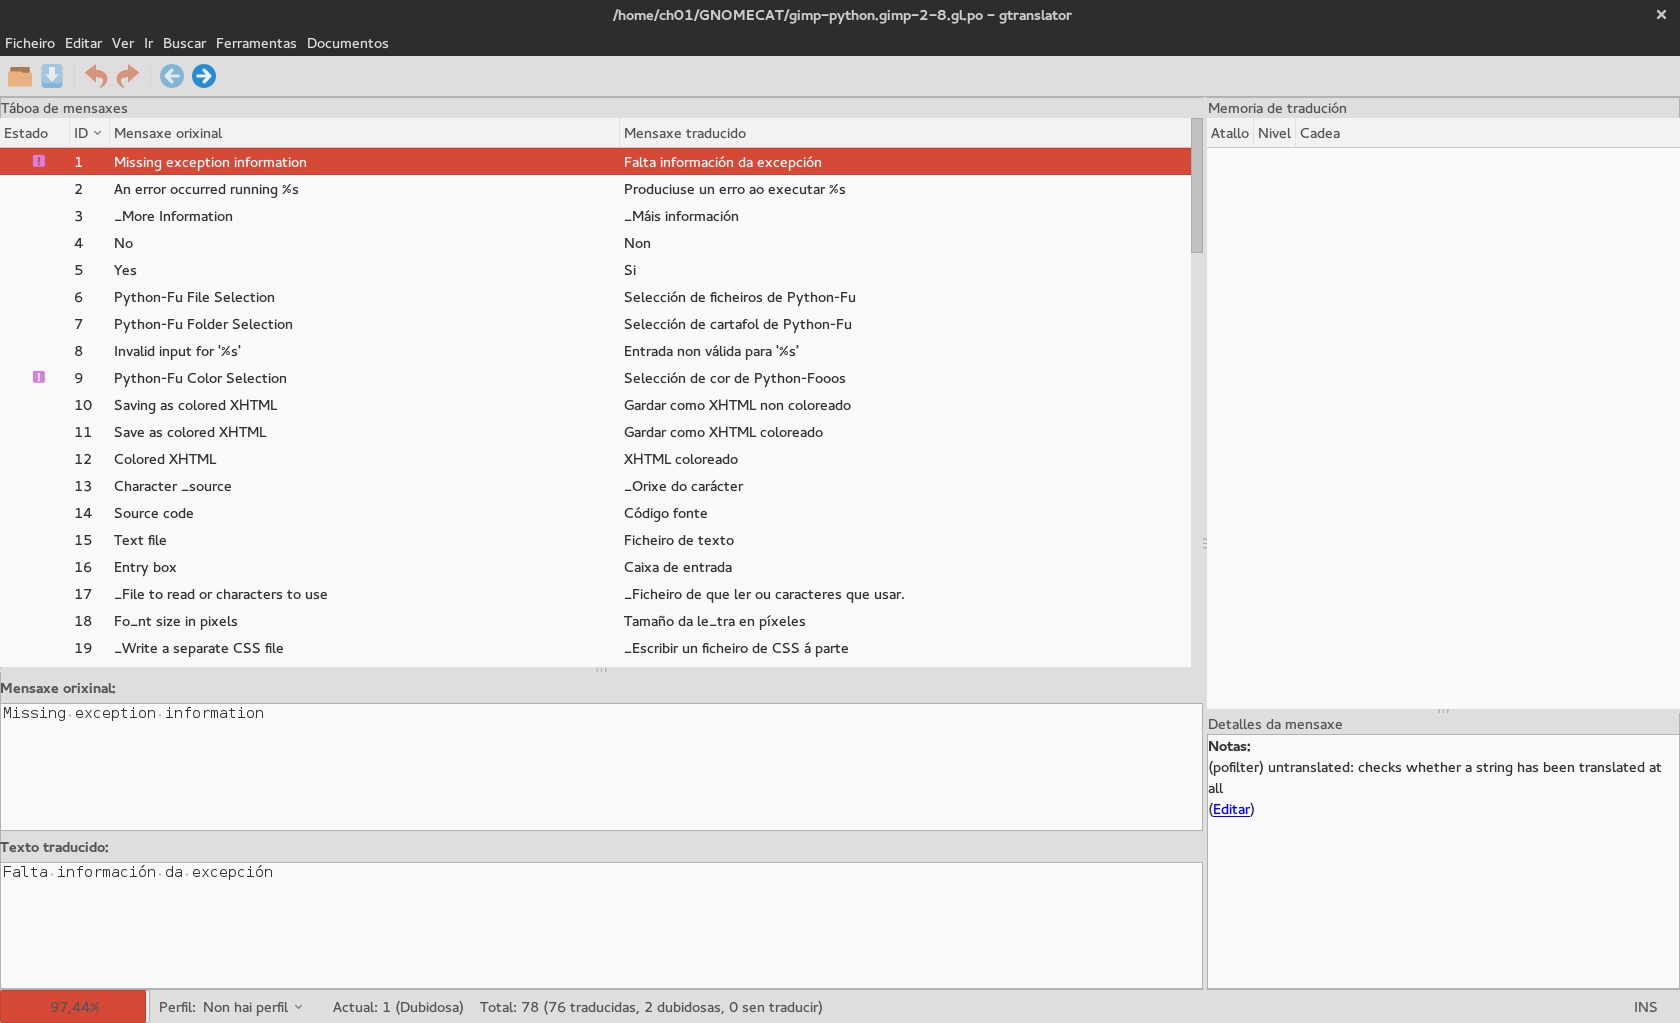
\includegraphics[width=\textwidth]{img/captura_gtranslator.png}
    \caption[Interface de GTranslator]{Interface de GTranslator}
    \label{fig:gtranslator}
\end{figure}

En canto a interface, como podemos ver na Figura~\ref{fig:gtranslator}, a parte máis importante do programa é a a lista de mensaxes. Abaixo desta lista temos un panel onde se pode editar cada mensaxe e a súa dereita a memoria de tradución. A disposición dos elementos desta interface é configurable xa que permite mover e ampliar cada un dos módulos. O programa tamén incorpora atallos de teclado que permiten moverse polo documento e seleccionar cada elemento da memoria de tradución.

Este programa pese a ser o aplicativo oficial de GNOME é moi pouco usado. As razóns disto son a ausencia dunha característica chave que o diferencie doutras ferramentas do mercado, a presencia de fallas importantes que afectan a usabilidade e a ausencia dun mantedor que resolva estes problemas.

\subsection{Lokalize}
Lokalize é o programa oficial para o soporte a tradución en KDE. Foi escrita dende cero empregando a tecnoloxía de KDE Platform 4 e baseándose no código de KBabel. As súas características máis destacables son, o soporte para ficheros GNU Gettext e o formato QT TS entre outros; a xestión de proxectos incorporando unha vista que permite ver un resumo de cada ficheiro dentro do proxecto; uso de memorias de tradución e de glosarios; comprobación da ortografía e vista previa das traducións a partir de scripts feitos polo usuario.

\begin{figure}[h]
    \centering
    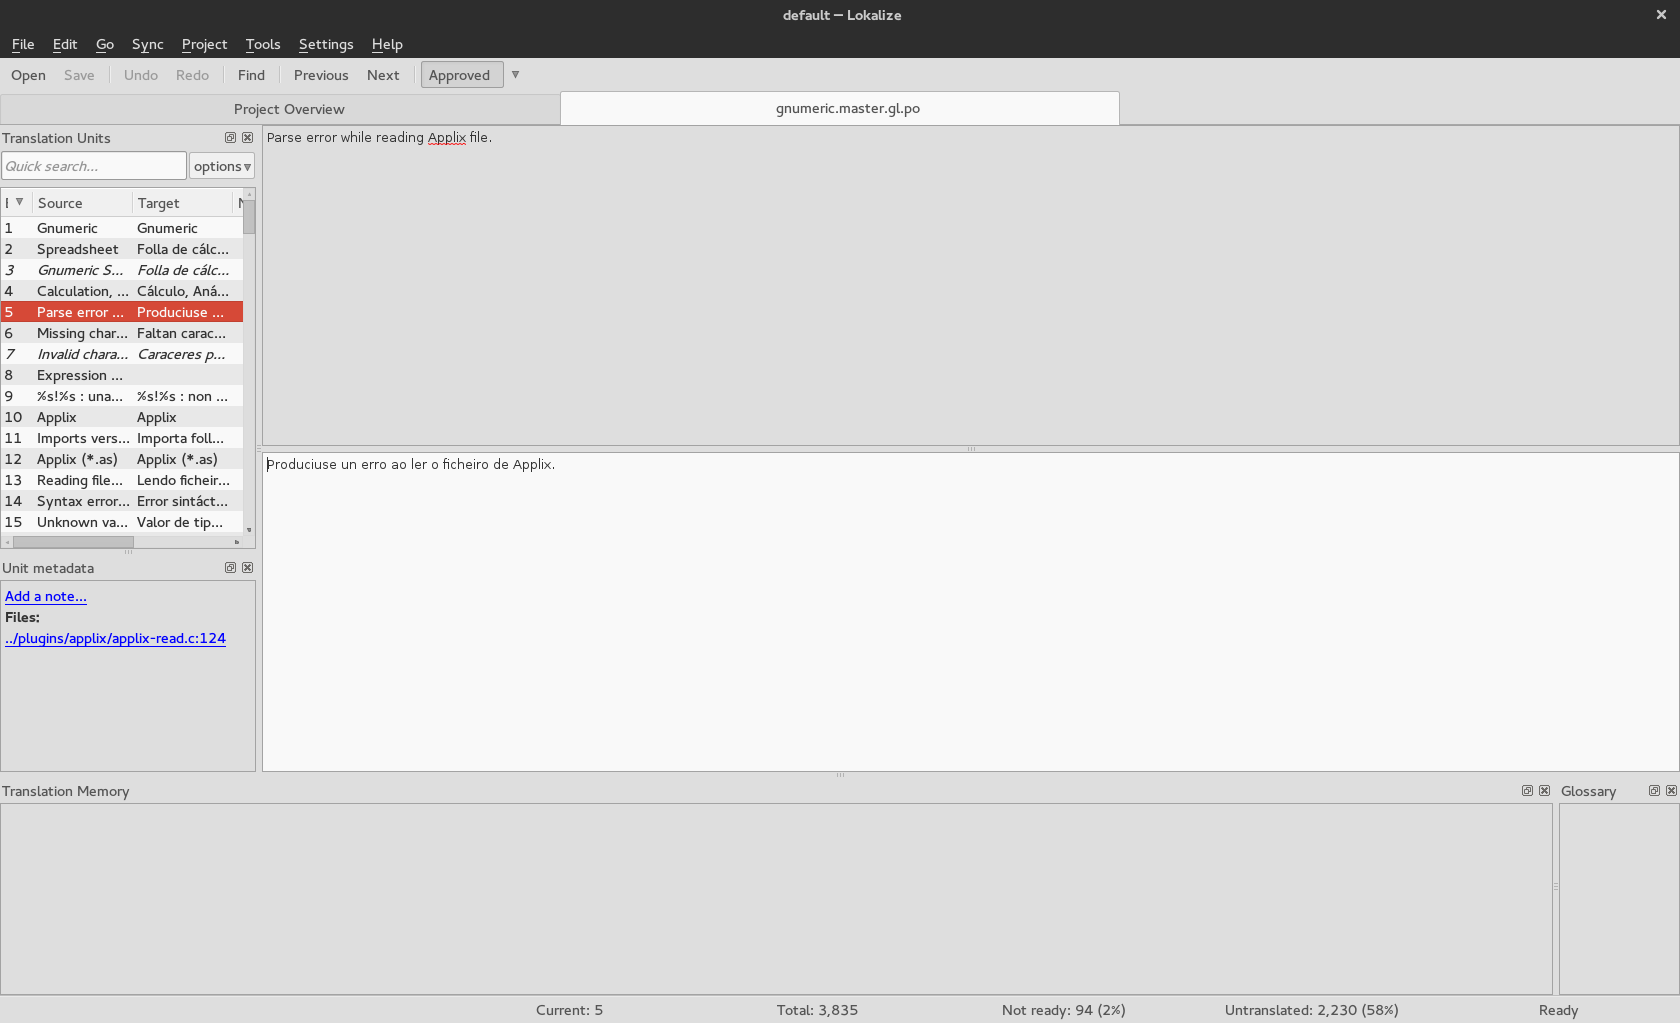
\includegraphics[width=\textwidth]{img/captura_lokalize.png}
    \caption{Interface de Lokalize}
    \label{fig:lokalize}
\end{figure}

En canto a interface, o programa permite abrir varios ficheiros cada un na súa lapela. Como se pode ver na Figura~\ref{fig:lokalize}, a vista de tradución está centrada no panel de edición, onde aparecen tanto a cadea orixinal como a cadea a traducir. Na columna da esquerda podemos ver a lista de cadeas onde se amosan os primeiros caracteres da cadea orixinal e da tradución e o estado desta tradución. Ademais tamén se pode ver o contexto da tradución, engadir un novo comentario e ver en que ficheiros estaba dita tradución. Por último tamén podemos ver na parte inferior a memoria de tradución e o glosario.

\subsection{Virtaal}

Virtaal é unha ferramenta CAT creada por Translate House\footnote{Compañía que surxiu a partir dunha comunidade de tradutores de Sudáfrica e que está especializada na creación de ferramentas e bibliotecas para axudar a tradución.} As características máis destacables son a incorporación de suxestión a tradución, comprobación da calidade das tradución e, sobretodo, a capacidade de abrir unha gran variedade de formatos a través da biblioteca Translate Toolkit.

\begin{figure}[h]
    \centering
    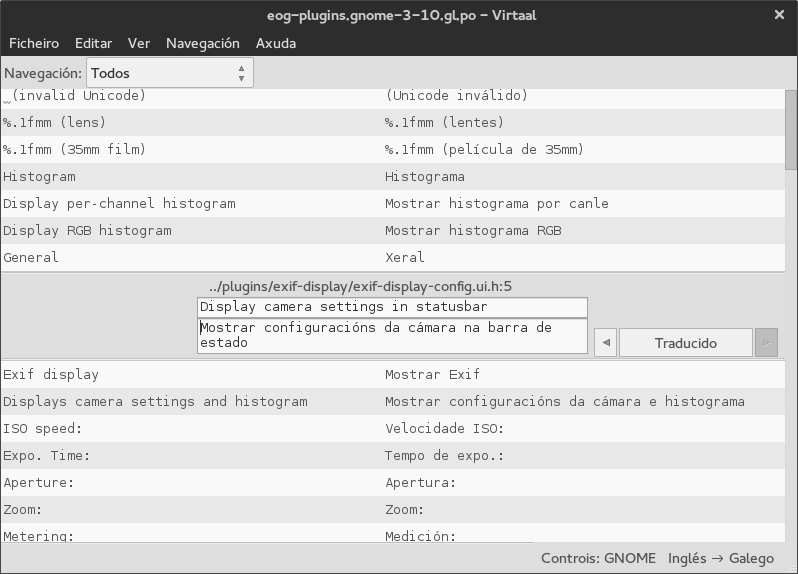
\includegraphics[width=\textwidth]{img/captura_virtaal.png}
    \caption{Interface de Virtaal}
    \label{fig:virtaal}
\end{figure}

Como se pode ver na Figura~\ref{fig:virtaal}, a interface é minimalista e moi centrada na tradución. A diferencia dos casos anteriores, trátase dunha interface fixa e que integra a lista das mensaxes coa edición da propia mensaxe. Tamén se indican posibles fallos que poidan ter a tradución, como falta de puntos o final, ausencia de marcadores de formato, etc.

\subsection{OmegaT}
Ferramenta CAT lanzada no ano 2001 e pensada fundamentalmente para tradutores profesionais. Ten soporte para o uso de memoria de tradución, glosario, tradución directa entre outras cousas. Destaca a gran cantidade de formatos que pode empregar.

\begin{figure}[h]
    \centering
    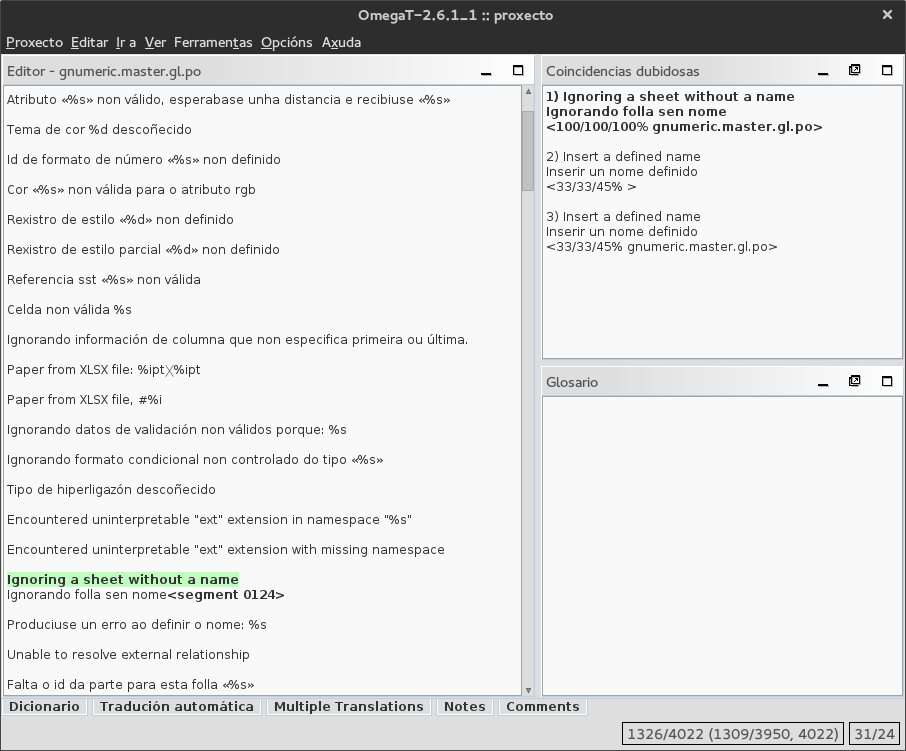
\includegraphics[width=\textwidth]{img/captura_omegat.png}
    \caption{Interface de OmegaT}
    \label{fig:omegat}
\end{figure}

A interface de OmegaT dista bastante do resto de programas. Como amosa a Figura~\ref{fig:omegat} non existe o concepto de lista de mensaxes traducir. O documento amosase como unha sucesión de cadea e se facemos clic encima dunha, permitiranos traducila. Trátase dun programa moi usado para a tradución tanto profesional como amateur.

\subsection{Google Translation Toolkit}
É a ferramenta CAT desenvolvida por Google e lanzada no ano 2008. A diferencia dos aplicativos analizados anteriormente, esta trátase unha solución puramente web. Entre as súas principais características encontrase a posibilidade de facer tradución automática empregando Google Translator, o uso de memorias de tradución compartidas, glosarios, soporte de etiquetas HTML entre outros e atallos de teclado. Ten soporte para varios formatos como ficheiros PO, documentos de Microsoft Word, de LibreOffice ou mesmo artigos da Wikipedia.

\begin{figure}[h]
    \centering
    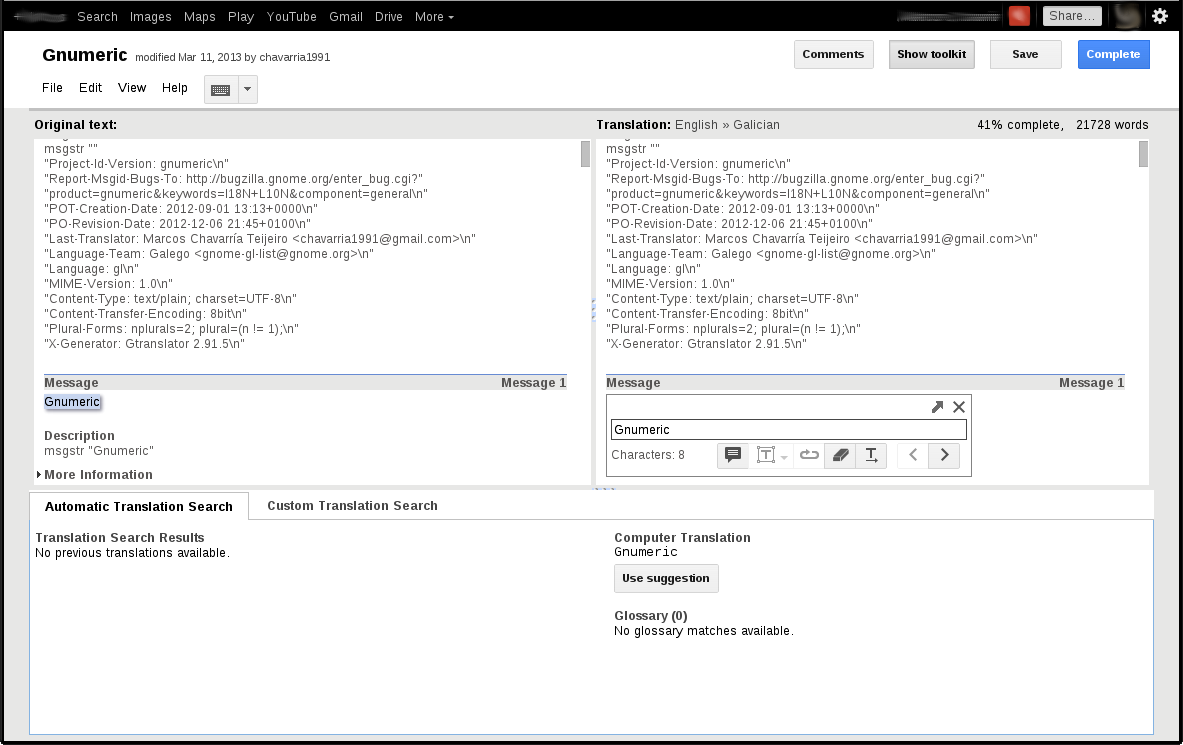
\includegraphics[width=\textwidth]{img/captura_googletranslationtoolkit.png}
    \caption{Interface de Google Translation Toolkit}
    \label{fig:translatetoolkit}
\end{figure}

Como se pode ver na Figura~\ref{fig:translatetoolkit}, na interface misturase a lista de cadeas co cadro de edición das mesmas. Ademais empregando unha interface semellante a do resto de ferramentas ofimáticas de Google, temos botóns para autocompletar tags e para avanzar a seguinte tradución. Aínda que foi pensado para a tradución colaborativa de documentos de ONGs e artigos da Wikipedia, na actualidade emprégase maioritariamente para a tradución de proxectos comerciais.


\subsection{Transifex}
Trátase dunha plataforma que xurdiu a partir dun proxecto do Google Summer of Code do ano 2007 que pretendía crear unha plataforma online máis amigable que o Damned Lies de GNOME que naquel momento tamén empregaba Fedora unha distribución de GNU/Linux. Trátase dunha solución de pago con plans que van dende os 19 a os 300 dólares. Non obstante os proxectos de código aberto poden usar o servizo de forma gratuíta e dispón de un período de mostra 30 días. As súas principais características son a posibilidade de descargar o documento e volvelo a subir para poder traducilo con outra ferramenta CAT, editor online, memoria de tradución e unha API que permite integralo con outros servizos. Ademais tamén soporta unha gran variedade de formatos entre os que se atopan os ficheiros PO, DTD de Mozilla ou XML entre outros.

\begin{figure}[h]
    \centering
    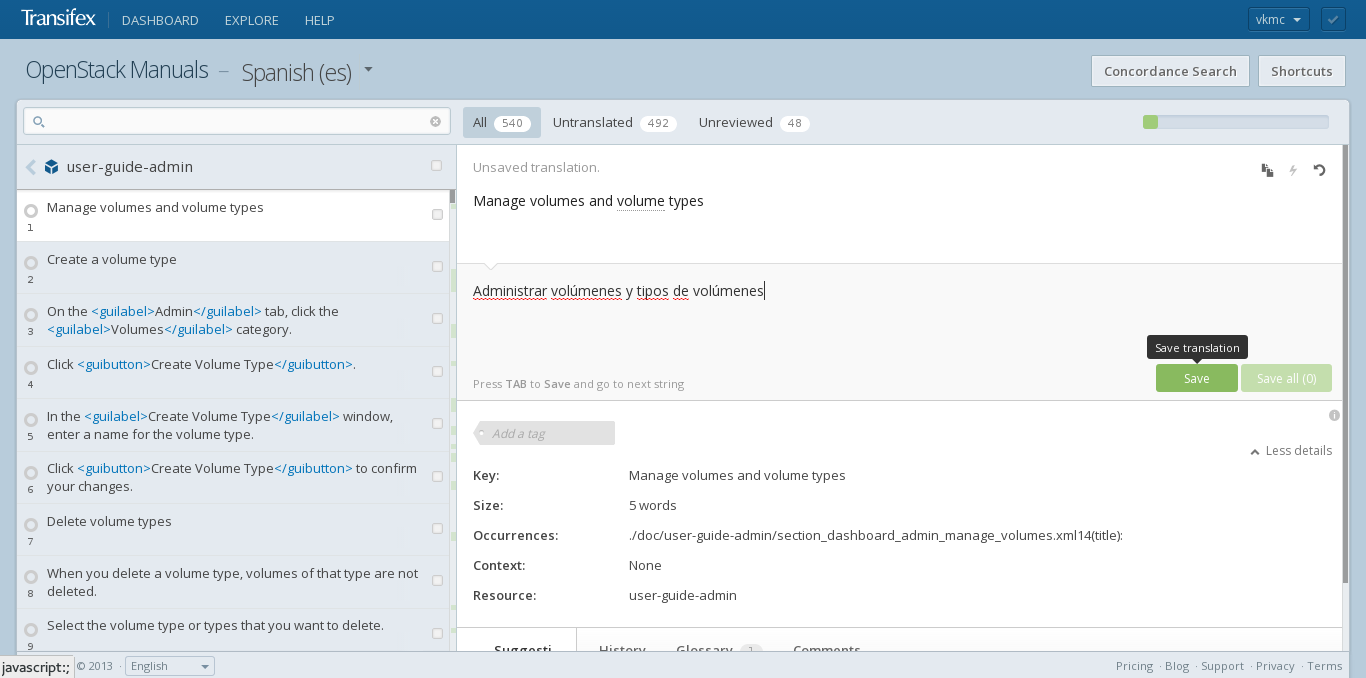
\includegraphics[width=\textwidth]{img/captura_transifex.png}
    \caption{Interface de Transifex}
    \label{fig:transifex}
\end{figure}

A interface de trasifex, como ser pode ver na Figura~\ref{fig:transifex} separa a lista de cadeas do cadro de edición. No cadro de edición temos a posibilidade de consultar a memoria de tradución ou o glosario. O programa tamén incorpora resaltado de sintaxe.

\subsection{Outras ferramentas}
Existen moitas máis ferramentas CAT no mercado. De feito, segundo unha enquisa \cite{article:2006survey} elaborada polo Imperial College London a cerca de 900 tradutores profesionais de 54 países diferentes, os únicos programas de todos os anteriores que aparecen citados é o OmegaT que conta con un 7\% de usuarios. As ferramentas máis usadas son ferramentas para Microsoft Windows e ferramentas con licencias privativas e usualmente moi caras. Algunhas destas ferramentas son TRADOS, Wordfast, DejaVu SDLX ou STAR Transit. Na Figura~\ref{fig:enquisa2006} podemos ver unha gráfica coas ferramentas máis empregadas segundo este estudio.

\begin{figure}[h]
    \centering
    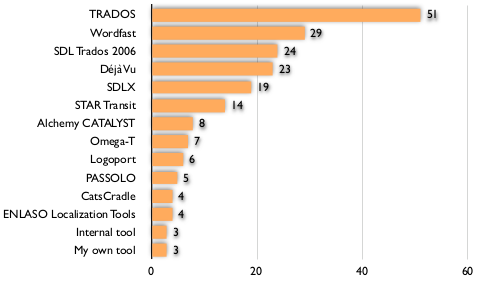
\includegraphics[width=0.7\textwidth]{img/grafico_uso_cat_enquisa2006.png}
    \caption{Ferramentas CAT máis empregadas segundo \cite{article:2006survey}.}
    \label{fig:enquisa2006}
\end{figure}

Hai que ter tamén en conta que se trata dun estudio bastante antigo polo que algunhas das ferramentas analizadas aínda non existían. Por exemplo a enquisa cita a ferramenta KBabel, que é a ferramenta de KDE na que está baseada Lokalize, pero con menos dun 2\% de usuarios.


\section{Características xenéricas das ferramentas CAT}

Algunhas das características que aparecen de forma recurrente en todas as ferramentas analizadas son as seguintes:

\subsection{Memoria de Tradución}
Unha memoria de tradución é unha base de datos composta de textos orixinais acompañados das súas traducións. Estes textos almacénanse en segmentos onde a separación entre segmentos ven dada por signos de puntuación ou o cambio de parágrafo, sendo esta última forma a máis frecuente.

A principal función dunha memoria de tradución e a extracción de coincidencias totais ou parciais. Os programas que teñen esta característica buscan na base de datos un segmento que coincida de forma exacta ou parcial coa cadea que se está a traducir e mostrase este segmento como suxerencia. Xunto coa suxerencia tamén se amosa o grado de cercanía entre a cadea a traducir e a cadea da memoria de tradución.

Existe un formato estándar de compartición de memorias de tradución de nome Translation Memory eXchange (TMX) e plataformas online que almacenan gran cantidade de cadeas e polo tanto hai máis posibilidade de obter unha mellor coincidencia. O software Amagama creado por Translate House, os creadores de Virtal, é un exemplo de memoria de tradución online.

\subsection{Glosario}
Un glosario é unha base de datos de termos xunto con unha ou varias traducións aceptadas. Diferenciase da memoria de tradución en que so se proporcionan a tradución a termos e non a cadeas completas. De igual forma que no caso das memorias de tradución, existe un formato estándar de para a compartición de glosarios de nome TermBase eXchange (TBX) e plataformas online para almacenar os glosarios.


\subsection{Previsualización}
As funcións de previsualización permítenlle ó tradutor ver como vai quedar a cadea traducida no programa final.

Os programadores e deseñadores fan as interfaces tendo en conta a lingua orixinal e non ningunha das traducións polo que se unha tradución é moito máis longa ca orixinal pode verse mal no programa final.

Para conseguir esta característica pódense empregar varias técnicas:

\begin{itemize}
  \item \textbf{Programa orixinal.} Esta técnica que se pode empregar en calquera cadea consiste en compilar o ficheiro PO e executar o programa final con ese ficheiro PO. Desta poderemos ver como queda a nosa tradución para o usuario final. A desvantaxe deste método consiste en que teremos que saber en que parte do programa se emprega a cadea que queremos previsualizar. Este método é empregado por Lokalize que permite a definición de scripts para a previsualización de cadeas.

  \item \textbf{Renderizado de interfaces de usuario en XML.} Nas bibliotecas de interfaces modernas existe a posibilidade de definir interfaces en ficheiros XML e despois renderizalas. Neste caso as cadeas a traducir van nestes arquivos e sería posible renderizar esta interface coa tradución que estamos a realizar. Este método aínda que si que amosaría a pantalla onde aparece a cadea actual, so é válido para as cadeas que proveñen destes ficheiros XML e non as definidas da forma tradicional. Un exemplo deste método pódese ver na rede no aplicativo Deckard\footnote{\href{http://deckard.malizor.org/}{deckard.malizor.org}} que permite ver as traducións de aplicativos de GNOME.
\end{itemize}


\subsection{Tradución Directa}
A tradución de cadeas de forma automática empregando algoritmos deseñados a tal proceso e que empregan grandes bases de datos aloxadas, xeralmente en internet. Tanto Google como Microsoft teñen os seus produtos corporativos que fan traducións e existen alternativas libres como OpenTrad ou Apertium. Estas traducións aínda que validas soen ser de baixa calidade polo que necesitan unha revisión.

	\chapter[An�lise de Requisitos]{An�lise de Requisitos globais}

Proin sit amet est. Nunc vel sem sed ligula accumsan cursus. Nunc tincidunt purus non elit accumsan vestibulum. Proin ultrices metus non nisl. Duis feugiat enim et sapien. Suspendisse lectus. Aliquam erat volutpat. Vestibulum ullamcorper. Nullam augue urna, pharetra nec, feugiat at, pellentesque a, nibh. Curabitur nulla.


%
% SECCION - T�tulo de la secci�n
%
\section[Nullam ante lorem placerat et]{
	Nullam ante lorem placerat et\footnote{Ejemplo de pie de p�gina desde un t�tulo de secci�n.}
}


Vestibulum pretium, libero in cursus posuere, metus nisi viverra libero, sed luctus arcu orci ac purus. Nulla tristique. Aliquam erat volutpat. Morbi in quam at neque egestas ultricies. Sed tempor consectetuer metus. Aliquam erat volutpat. Duis non tortor a quam tristique ultricies. Aenean eget augue eget nisi rutrum commodo. Vestibulum bibendum pellentesque lectus. Praesent et mauris a urna ultricies scelerisque. Class aptent taciti sociosqu ad litora torquent per conubia nostra, per inceptos himenaeos.

Nulla purus est, venenatis eget, hendrerit vitae, lacinia eget, dui. Maecenas tincidunt augue vel mi. Lorem ipsum dolor sit amet, consectetuer adipiscing elit. Fusce eu erat nec nisl pellentesque facilisis. Donec porttitor. Sed in nisl. Sed tristique tincidunt ipsum. Sed nec lectus. Quisque blandit, neque ut ullamcorper imperdiet, nibh justo imperdiet pede, sit amet egestas erat enim quis urna. In non urna eu lectus varius consequat. Nam interdum. Sed in metus vel enim ornare congue. Curabitur pede. Curabitur rutrum. Vestibulum ante ipsum primis in faucibus orci luctus et ultrices posuere cubilia Curae; Sed dui mauris, iaculis a, lobortis vitae, rhoncus id, nibh. Phasellus leo velit, dapibus quis, ultrices vitae, hendrerit sit amet, velit. Maecenas pretium pellentesque pede. Sed rutrum aliquet massa. Maecenas tellus.

\begin{sidewaystable}
	\begin{center}
		\begin{tabular}{|c|c|c|c|c|c|c|c|c|c|c|c|c|c|}
			\hline
				\multirow{5}{1cm}{\scriptsize{\textbf{Tramo}}}	&
				\multirow{4}{0.15cm}{\scriptsize{\textbf{a}}}	&
				\multirow{4}{1.25cm}{\scriptsize{\textbf{Desnivel}}}	&
				\multicolumn{11}{|c|}{\scriptsize{Temperatura (\textdegree C)}}\\
			\cline{4-14}
				&
				&
				&
				\scriptsize{-5} &
				\scriptsize{5} &
				\scriptsize{10} &
				\scriptsize{15} &
				\scriptsize{20} &
				\scriptsize{25} &
				\scriptsize{30} &
				\scriptsize{35} &
				\scriptsize{40} &
					\scriptsize{45} &
					\scriptsize{50} \\
				\cline{4-14}
					&
					&
					&
					\multicolumn{11}{|c|}{\scriptsize{Tense (daN)}}\\
				\cline{4-14}
					&
					&
					&
					\scriptsize{$275.38$} &
					\scriptsize{$221.57$} &
					\scriptsize{$199.4$} &
					\scriptsize{$180.4$} &
					\scriptsize{$164.32$} &
					\scriptsize{$150.78$} &
					\scriptsize{$139.38$} &
					\scriptsize{$129.74$} &
					\scriptsize{$121.54$} &
					\scriptsize{$114.5$} &
					\scriptsize{$108.4$} \\
				\cline{4-14}
					&
					\scriptsize{(m)} &
					\scriptsize{(m)}	&
					\multicolumn{11}{|c|}{\scriptsize{Flecha (m)}}\\
				\hline
				\hline
					\scriptsize{1-2} &
					\scriptsize{80}	&
					\scriptsize{$11.09$}	&
					\scriptsize{$0.55$} &
					\scriptsize{$0.68$} &
					\scriptsize{$0.75$} &
					\scriptsize{$0.83$} &
					\scriptsize{$0.91$} &
					\scriptsize{$1.00$} &
					\scriptsize{$1.08$} &
					\scriptsize{$1.16$} &
					\scriptsize{$1.24$} &
					\scriptsize{$1.31$} &
					\scriptsize{$1.39$} \\

				\hline
		\end{tabular}
	\end{center}
	\caption[Ejemplo de tabla rotada]{Tabla rotada para aprovechar la altura de la p�gina.}
	\label{cuadro_regulacion_1_2}
\end{sidewaystable}

Donec a pede. Proin dolor. Ut nunc ligula, tempor id, ornare sit amet, aliquam et, nibh. In mollis iaculis pede. Vivamus gravida orci eu nisl. Sed nibh sem, consequat at, iaculis non, placerat in, ligula. Praesent id nisi. Nunc pellentesque justo non libero. Sed quis est sit amet purus lobortis blandit. Sed arcu justo, rhoncus condimentum, ullamcorper iaculis, viverra et, nisl. Mauris leo risus, placerat sit amet, commodo eget, lacinia at, ipsum. Fusce vulputate suscipit ipsum.



%
% SECCION - T�tulo de la secci�n
%
\section[�Nunc vel turpis ut varius vehicula est sed pulvinar?]{
	�Nunc vel turpis ut varius vehicula est?
}

Nunc vel turpis. Ut varius vehicula est. Sed pulvinar. Aliquam vehicula quam vitae sapien. Cras eget lectus a metus tempor venenatis. Phasellus et nulla. Class aptent taciti sociosqu ad litora torquent per conubia nostra, per inceptos himenaeos. Etiam sodales nibh aliquam dolor. Donec pulvinar lobortis risus. Ut augue erat, hendrerit a, accumsan non, elementum porttitor, est. Sed tincidunt neque nec ligula. Donec enim sapien, dictum gravida, porta non, molestie eu, lectus. Sed ultrices lectus at sem. Cras suscipit tortor id dolor. Nullam lacus risus, blandit non, lobortis sed, dignissim ut, nibh. Sed neque. Phasellus ullamcorper orci quis magna.

\begin{itemize}
	\item{
		�tem 1: Nam commodo ligula eget lorem. Nullam consectetuer nibh id orci. Aliquam ornare nisl nec risus. Quisque quis nunc. In ullamcorper, enim in eleifend aliquet, ipsum felis ultricies nibh, eu aliquam libero libero a lorem. Curabitur fringilla, massa nec vestibulum viverra, purus nulla ultricies ante, vitae dignissim tortor purus at dui. Fusce quis nisi. Aliquam erat volutpat. Sed molestie ultricies nunc. Nam vitae eros eget nibh tristique suscipit. Morbi ut velit. Quisque quis nulla a ipsum malesuada fermentum.
	}
	\item{
		�tem 2: Fusce scelerisque tortor ac libero. Class aptent taciti sociosqu ad litora torquent per conubia nostra, per inceptos himenaeos. Quisque nec est. Nunc ut risus a arcu congue ultricies. Aenean laoreet dapibus orci.
	}
	\item{
		�tem 3: Sed gravida dui et eros. Praesent id lacus. Etiam velit libero, tristique tempus, facilisis quis, bibendum euismod, magna. Quisque ut mi. Nam quis ipsum. Nulla porta dapibus arcu. Nullam ut purus vel libero scelerisque sodales.
	}
\end{itemize}

Aenean vitae sem nec turpis sagittis egestas. Sed nisi sapien, rutrum sit amet, dictum id, pretium eget, libero. Donec viverra risus eget mi. Duis porttitor. Nunc et sem eu augue dapibus condimentum. Mauris a tortor vel est adipiscing malesuada. Morbi neque mauris, vestibulum at, tincidunt vitae, convallis nec, ligula. Vestibulum quis turpis.



%
% SECCION - T�tulo de la secci�n
%
\section[Aenean sit amet lorem a dui sagittis tincidunt]{
	Aenean sit amet lorem a dui sagittis tincidunt
}
\label{ejemplo_etiqueta_para_referenciar_seccion_020}

Lorem ipsum dolor sit amet, consectetuer adipiscing elit. Nunc varius ornare mauris (ver cuadro \ref{ejemplo_referencia_a_tabla_020}). Donec orci quam, mattis eu, gravida in, condimentum eget, lacus. Integer a enim. Pellentesque turpis purus, feugiat in, dictum ut, interdum ut, nulla. Mauris purus.


% TODO: Tiene que haber alguna manera de hacer que la separaci�n entre la tabla y el p�rrafo sea configurado en el pre�mbulo...
\vspace{0.5cm}
\begin{table}[h]
	\begin{center}
		\begin{tabular}{lp{6cm}rr}
			\toprule
				% CABECERA
				Animal &
				Description &
				Quantity &
				Price (\$) \\
			\midrule
			\midrule
				% FILA 1
				Gnat &
				Colloquial name to any of various small insects &
				10 &
				13.65 \\

				% FILA 2 (con las dos primeras columnas en blanco)
				&
				&
				100 &
				6.00 \\

				% FILA 3
				Gnu &
				An antelope of the genus Connochaetes &
				1 &
				92.50 \\

				% FILA 4
				Emu &
				The largest bird native to Australia &
				2 &
				33.33 \\

				% FILA 5
				Armadillo &
				Small placental mammals, known for having a bony armor shell &
				1 &
				8.99 \\
			\bottomrule
		\end{tabular}

	\end{center}

	\caption[Ejemplo de cuadro o tabla]{Ejemplo de cuadro o tabla.}
	\label{ejemplo_referencia_a_tabla_020}

\end{table}


% Subsecci�n
\subsection*{Donec consectetuer venenatis turpis}
Quisque enim neque, porta aliquam, tincidunt sed, eleifend quis, velit. Praesent sapien augue, suscipit nec, sodales a, faucibus in, mi. Ut et leo molestie massa elementum fringilla. Morbi sollicitudin sem vitae tortor tincidunt elementum. In ac nunc. Quisque placerat faucibus tellus. Nullam scelerisque, nibh et venenatis hendrerit, est diam semper mi, eu fringilla turpis augue vitae lectus. Ut accumsan mi at turpis. Sed sit amet magna eget augue vulputate blandit. Integer porttitor egestas nisl. Vestibulum consectetuer.

Quisque aliquet accumsan mauris. Nulla ante risus, semper eget, egestas sed, tristique vitae, arcu. Integer consequat dolor eget quam. Lorem ipsum dolor sit amet, consectetuer adipiscing elit. Donec consectetuer venenatis turpis. Etiam pharetra nisl vitae leo. Ut vehicula interdum leo. Donec in nisi. Morbi sagittis eleifend quam. Sed scelerisque mi at justo. Aliquam erat volutpat. Nulla consequat porttitor eros.


% Subsecci�n
\subsection*{Duis vestibulum risus vitae sem}
Suspendisse malesuada aliquam nunc. Integer neque. Nulla in magna. Duis vestibulum risus vitae sem. Morbi eu nunc sit amet erat facilisis pellentesque. Duis scelerisque risus vitae magna. Suspendisse placerat est eget lectus tristique tincidunt. Maecenas dolor nunc, vehicula in, vestibulum nec, varius a, sapien. Suspendisse in felis et ipsum tempor adipiscing. Cras elementum nulla vel lorem. Aliquam fringilla pharetra nulla.

Aenean et lectus sed orci consequat faucibus. Nunc neque velit, feugiat at, iaculis at, ullamcorper nec, ligula. Sed laoreet, ipsum id iaculis bibendum, ipsum nibh bibendum urna, ut blandit arcu nisl blandit odio. Donec eros lorem, luctus at, ultrices sed, facilisis sed, est. Maecenas pharetra, felis a tempus aliquet, magna elit auctor lectus, eget euismod quam leo sit amet nibh. Ut commodo. Aliquam enim tellus, sodales vel, bibendum a, lacinia sed, metus. Nullam sed ligula ac libero rutrum molestie. Aliquam suscipit, eros non aliquet feugiat, magna mauris elementum pede, nec tristique nisl lorem hendrerit orci.


% Subsecci�n
\subsection*{Mauris molestie}
Aliquam vehicula purus id quam. Pellentesque egestas. Mauris molestie. Duis in arcu quis turpis elementum interdum. Curabitur eu orci. Nulla rhoncus convallis quam. Donec volutpat eleifend turpis. Ut nulla magna, hendrerit nec, laoreet ac, malesuada et, nisl. In dolor. Donec elit. Maecenas laoreet, eros non lobortis faucibus, turpis nisi viverra pede, vel ullamcorper pede tortor vel ligula.

Sed porttitor tincidunt mauris. Sed tempus libero sed turpis. Curabitur dictum adipiscing mi. Nunc porta leo quis nunc. Nunc euismod. Integer eu sem. Integer dapibus libero et eros. Mauris nisi. Quisque iaculis cursus enim (ver figura~\ref{ejemplo_referencia_a_figura_020}). Donec ut diam. Pellentesque erat.


% Incluimos una figura...
\begin{figure}[h]
	\centering
	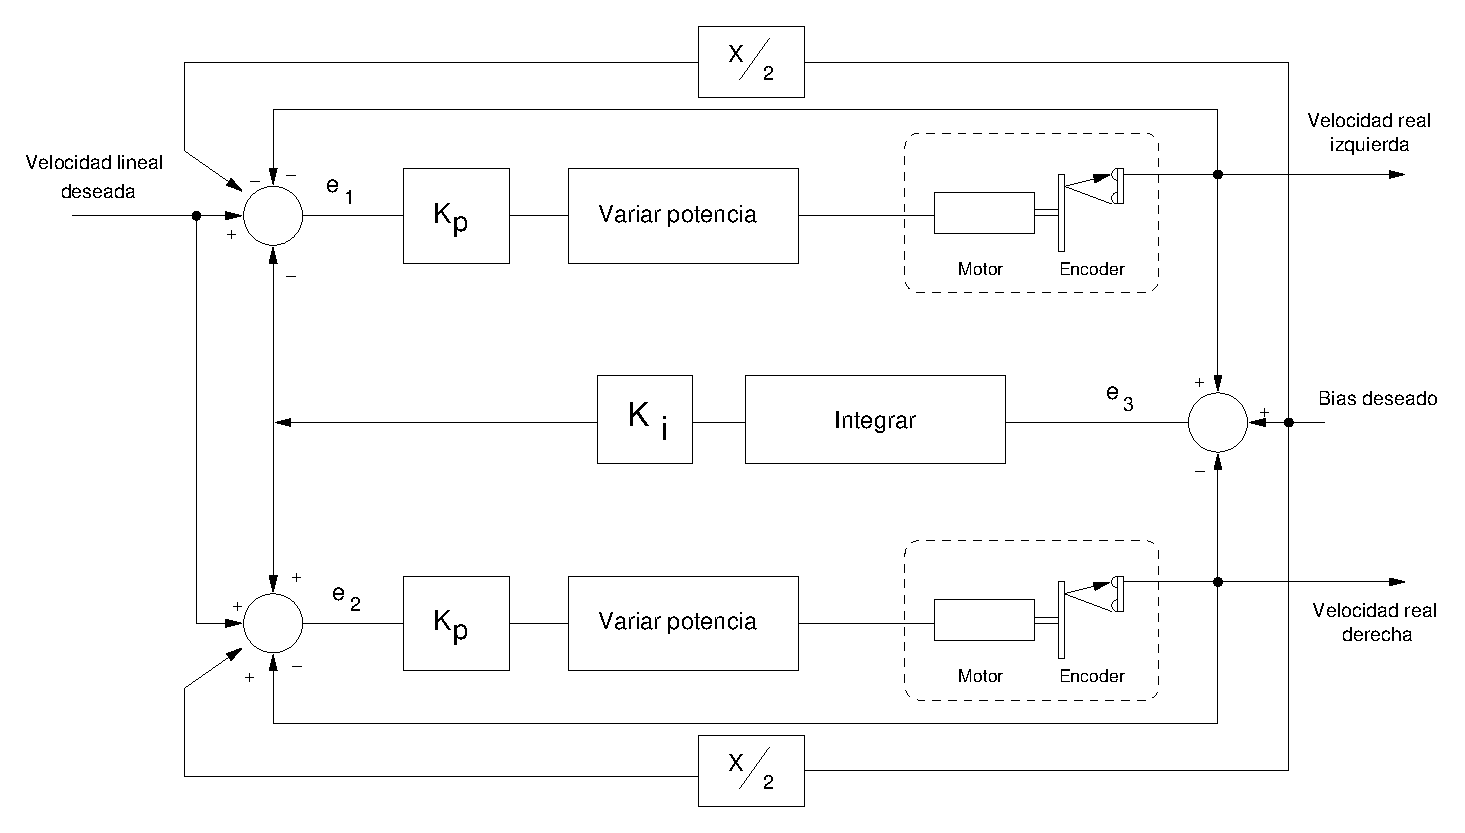
\includegraphics[width=10cm]{./eps/control-pi.eps}
	\caption[Ejemplo de inclusi�n de figura o imagen]{
		Ejemplo de inclusi�n de figura o imagen.
	}
	\label{ejemplo_referencia_a_figura_020}
\end{figure}



%
% SECCION - T�tulo de la secci�n
%
\section[Praesent purus sem]{
	Praesent purus sem
}

Fusce fringilla feugiat turpis. Fusce bibendum. Quisque a magna. Aenean dignissim sollicitudin eros. Proin posuere vulputate nibh. Morbi nec diam vitae velit blandit tincidunt. Suspendisse in nisi sit amet ipsum luctus fringilla.


\paragraph*{Ut sed urna.}
Vivamus fermentum. Nulla eget lectus vel ligula dignissim condimentum. Fusce tristique, eros sit amet tempor congue, urna diam fermentum enim, ac ullamcorper urna magna ac ligula. Donec ultrices neque eu purus. Integer vehicula, mi eget mollis vehicula, risus tellus pulvinar dolor, a fringilla dui mauris sit amet leo. Nulla vestibulum est ut est.

\paragraph*{Vivamus eu dui.}
Nulla tempus augue a sapien. Etiam non nibh. In lacus libero, ullamcorper eget, feugiat eu, tincidunt in, orci. Vivamus leo dolor, vehicula id, tempus et, venenatis at, dui. Pellentesque convallis ligula ut dui. Cras eu dolor sed dui tincidunt congue. Suspendisse justo elit, laoreet nec, fermentum id, lacinia viverra, lectus. Fusce erat velit, placerat id, dignissim et, gravida vitae, odio. Quisque massa enim, varius quis, pellentesque vel, hendrerit sit amet, mauris.

\paragraph*{etiam blandit imperdiet orci.}
Sed tempor pede a neque. Donec sed massa. Nam ornare auctor enim. Nunc vitae erat. In turpis. Quisque quam tortor, interdum sit amet, dapibus ac, bibendum et, sapien. In malesuada auctor elit. Pellentesque habitant morbi tristique senectus et netus et malesuada fames ac turpis egestas. Vivamus dignissim ligula quis ante. Phasellus dolor massa, accumsan in, aliquam nec, scelerisque ac, sem. Nunc ac orci. Donec risus libero, elementum non, euismod sollicitudin, pharetra ac, nibh. Curabitur nisi est, gravida vel, vulputate id, faucibus non, nibh.

\paragraph*{Curabitur iaculis ante.}
Phasellus nunc arcu, sodales eu, ultrices sed, suscipit ac, nisl. Quisque at velit. Suspendisse lobortis urna non metus. Donec lacinia congue risus. Suspendisse tempus nibh vel metus. Mauris lacinia volutpat nibh. Integer vitae mauris. Cras placerat lobortis nibh. In nisl odio, convallis a, vulputate id, ultrices in, nunc.

\paragraph*{Morbi bibendum varius lorem.}
Curabitur eget sapien quis nulla fermentum iaculis. Vivamus elementum elit in ante. Nullam magna ipsum, semper quis, tempus sit amet, semper at, eros. In euismod molestie odio. Donec a ante. Morbi vel diam nec diam tincidunt luctus. Nunc rhoncus. Fusce metus justo, blandit facilisis, pulvinar eu, imperdiet sit amet, lectus.



%
% SECCION - T�tulo de la secci�n
%
\section[Vestibulum non lorem]{
	Vestibulum non lorem
}


Nam pellentesque, mauris eget mollis lobortis, lectus velit sollicitudin nulla, quis dapibus tortor mi in nibh. Cras viverra pede id augue. Ut sed urna ut pede rutrum vulputate. Sed pulvinar urna et eros. Proin cursus suscipit odio. Aenean aliquet. Nullam nibh ipsum, euismod facilisis, tincidunt eget, ultricies ut, turpis. Cras elementum. Proin vel eros vitae risus pretium aliquet. Sed sit amet purus in enim auctor iaculis. Curabitur pulvinar. Etiam in lectus sed enim egestas suscipit. Proin dignissim leo quis diam. Nam sed arcu eget velit vestibulum dapibus.

\paragraph*{Integer ornare.}
Suspendisse lacinia sollicitudin mauris. Vestibulum felis est, sollicitudin sit amet, sollicitudin eget, dignissim eget, odio. Curabitur tincidunt metus euismod eros. Quisque libero.

\paragraph*{Duis semper dolor mattis quam.}
Praesent a ligula a enim sollicitudin laoreet. Cras varius semper eros. Aliquam egestas, sapien accumsan malesuada blandit, nisl magna viverra tortor, nec porttitor dolor nisi sed pede. Ut non nulla nec est aliquet porta. Nulla nec diam. Ut in libero vitae turpis fringilla posuere. Aliquam vestibulum pulvinar orci. Quisque lacinia neque porttitor nisi. Cum sociis natoque penatibus et magnis dis parturient montes, nascetur ridiculus mus. Sed augue diam, feugiat sed, pulvinar non, tempus vel, nunc. Nulla facilisi. Aenean sed enim sit amet odio aliquet dictum. Nulla vel arcu. Donec sodales. Nunc purus. Morbi semper lobortis nibh. Proin id risus ut elit hendrerit consectetuer. Vestibulum eu risus.

\paragraph*{Lorem ipsum}
Etiam ante risus, egestas ut, suscipit vel, auctor vitae, metus. Mauris fermentum laoreet est. Cum sociis natoque penatibus et magnis dis parturient montes, nascetur ridiculus mus. Aenean porttitor magna eget arcu aliquam dictum.

Curabitur pulvinar. In tortor justo, malesuada at, ullamcorper a, tristique in, enim. Curabitur justo tellus, aliquet a, congue in, elementum quis, urna. Proin pulvinar enim a diam. Nunc adipiscing. Maecenas sodales elementum leo. Lorem ipsum dolor sit amet, consectetuer adipiscing elit. Proin et nisl non quam molestie consequat.

Aliquam adipiscing bibendum justo. Duis mi. Maecenas semper eros at nibh. Maecenas pharetra odio et quam. Donec ligula diam, sodales condimentum, varius nec, lacinia sed, urna. Vestibulum dignissim diam quis lectus vehicula imperdiet. Etiam ornare, odio id lacinia semper, libero quam rhoncus eros, sollicitudin sagittis nulla lacus non elit. Etiam ultricies mi nec leo.

\paragraph*{Curabitur eleifend libero sit amet odio.}
Curabitur sit amet orci at lacus euismod rutrum. Aliquam gravida venenatis nulla. Phasellus ligula. Praesent erat lorem, tincidunt id, ullamcorper et, egestas at, nulla. Cras sed dolor. Aliquam dignissim, nisl sit amet venenatis porttitor, erat nisl pharetra est, et hendrerit nisl odio nec elit. Cras consectetuer.


% subsecci�n
\subsection[Suspendisse sit amet elit]{Suspendisse sit amet elit}

Nam dui leo, suscipit ac, tincidunt ut, placerat eget, ipsum. Suspendisse feugiat volutpat ligula. Vestibulum ante ipsum primis in faucibus orci luctus et ultrices posuere cubilia Curae; Pellentesque vulputate molestie sem. Nullam porta odio et justo ultrices bibendum. Phasellus convallis vehicula mauris. Nunc cursus, elit in porta tincidunt, odio magna faucibus mi, ut pretium augue nisl a mi. Mauris quis massa.

\paragraph*{Nunc pharetra.}
Nisl a convallis eleifend, pede urna aliquet lacus, ut condimentum tellus lectus eu arcu. Nam tincidunt luctus nulla. Pellentesque suscipit, justo sed interdum sodales, tellus elit dapibus tellus, sed ultrices magna arcu a magna. Duis velit diam, semper sit amet, venenatis sed, lacinia id, ligula. Integer malesuada. Cum sociis natoque penatibus et magnis dis parturient montes, nascetur ridiculus mus. Suspendisse et mi a sapien euismod sagittis. Nulla facilisi. Proin a felis imperdiet enim facilisis mollis. Nunc lacus lectus, scelerisque nec, pretium in, ullamcorper sed, quam.



%
% SECCION - T�tulo de la secci�n
%
\section[Integer ullamcorper nulla facilisi]{
	Integer ullamcorper nulla facilisi
}

Nulla porttitor, ipsum non gravida eleifend, dolor est accumsan nulla, sit amet ultrices libero felis vitae leo. Vestibulum at dui id metus porttitor pretium. Praesent et justo. Pellentesque habitant morbi tristique senectus et netus et malesuada fames ac turpis egestas. Morbi ipsum nisl, adipiscing et, tempus sit amet, luctus ornare, metus. Aliquam tellus sem, commodo blandit, vehicula et, vulputate congue, tellus. Cum sociis natoque penatibus et magnis dis parturient montes, nascetur ridiculus mus. Vivamus hendrerit. Proin tincidunt dui id felis.

Vestibulum eu justo a dolor aliquam ultrices. Aenean lobortis sollicitudin justo. Donec semper. Suspendisse eros erat, condimentum id, aliquam ac, hendrerit vel, eros. Proin ac nulla rutrum eros sagittis hendrerit. Phasellus aliquet, purus ut rhoncus bibendum, turpis libero vehicula ante, eu lacinia erat augue pulvinar lorem. Integer pede. Mauris congue dui vel nisl. Aenean sodales, nisl vitae fermentum sollicitudin, nisl massa mollis diam, sit amet ultricies velit quam vitae dui. Etiam accumsan eros ut tellus. Nullam arcu nunc, porttitor tincidunt, varius vitae, pellentesque nec, turpis. Morbi suscipit pellentesque sem. Donec faucibus. Praesent congue. Curabitur elit. Nullam sed enim nec sem sagittis dictum. Ut sed justo eu elit gravida tincidunt. Phasellus convallis, augue vel iaculis euismod, turpis nisl tincidunt tortor, ut scelerisque pede nisi id ligula. Suspendisse sagittis, orci ac eleifend gravida, orci augue sodales velit, sed iaculis felis dui sit amet nisi. Vivamus tincidunt euismod purus.

Aenean semper neque eu lectus. Donec mollis ante sit amet libero. Curabitur nec enim ut arcu suscipit cursus. Nulla ac erat et mauris sollicitudin volutpat. Curabitur ornare sapien ut purus. In faucibus sapien at neque. Suspendisse sed arcu et quam aliquet tristique. Praesent sit amet elit vitae turpis lobortis hendrerit. Aliquam nec mi iaculis mi tempor tincidunt. Donec at nisl convallis magna ullamcorper mollis. Etiam pretium erat eget metus adipiscing aliquam. Donec faucibus, sem viverra porta vestibulum, magna mi ultricies erat, aliquet lobortis dui sapien ut purus. Fusce tellus pede, sodales in, ultrices non, commodo non, lorem. Sed at magna scelerisque nisl sollicitudin imperdiet. Vestibulum commodo, nisi id bibendum consequat, velit tellus ultricies justo, at consectetuer eros nulla at massa. In a magna sit amet purus viverra aliquet. Morbi vel sem ut turpis commodo pretium. Pellentesque dolor sem, tincidunt id, sollicitudin et, tincidunt et, sem.

Duis quam libero, viverra sed, cursus nec, facilisis ut, nulla. Phasellus eros lectus, sollicitudin ac, egestas non, tristique eget, nibh. Sed pharetra, sem a mattis pretium, lectus lacus gravida nibh, sit amet porta tortor ipsum nec sapien. Aenean ipsum. Nulla sit amet justo. Aliquam aliquet nibh in erat. Quisque auctor est vitae nibh. Proin in nisi. Sed imperdiet. Etiam urna justo, lacinia ut, dapibus eu, commodo at, nibh. Pellentesque quis tellus at diam sagittis convallis. Integer ac sapien eget odio sagittis aliquet. Phasellus sagittis.

Etiam non leo. Aliquam quis dui. Suspendisse suscipit dui at lacus. Curabitur id urna sed purus ullamcorper ullamcorper. Nullam ut sem eu sapien malesuada rhoncus. In leo urna, rhoncus vel, tempus quis, ultricies vitae, ipsum. Sed est justo, sodales a, semper et, pretium in, massa. Etiam aliquam est a ligula. Nullam eleifend scelerisque nisi. In sollicitudin mi vel nibh. Praesent dapibus, nisl quis tincidunt dictum, lorem quam dapibus lorem, tristique mollis mi tortor ut nulla. Sed sit amet sapien. Aenean non urna lacinia urna euismod interdum. Praesent in nibh. In mauris. Ut scelerisque lectus vitae neque.



%
% FIN DEL CAP�TULO
%
	\chapter{Metodoloxía}

Nesta sección descríbese a metodoloxía levada a cabo para a realización deste proxecto. Unha metodoloxía e un conxunto de métodos ou prácticas empregadas para a realización dunha tarefa, neste caso o analise, deseño e implementación dunha nova ferramenta CAT para o proxecto GNOME. Escolleuse unha metodoloxía axil de ciclo incremental. Moitas das prácticas que se tomaron son collidas da metodoloxía eXtreme Programming.

\section{eXtreme Programming}

Foi creada por Kent Beck no ano 1999 e trátase dun dos máis destacados métodos de desenvolvemento áxil. eXtreme Programming (a partir de agora XP) avoga por ciclos de desarrollo moi curtos e elimina os roles clásicos de analista, deseñador e programador. Todo equipo participa en todas as partes do desarrollo. Desta forma Beck define uns valores fundamentais da metodoloxía e unhas prácticas que axudan a adoptar estos valores.

\subsection{Valores de eXtreme Programming}

\subsubsection{Comunicación}
É o primeiro valor de XP. Segundo esta metodoloxía os problemas nos proxectos poden ser traducidos a alguén que non falou con outra persoa sobre algo importante do proxecto. Esta mala comunicación non sucede por casualidade e é debido frecuentemente as malas prácticas. Para solucionar isto, XP inclúe prácticas nas que é necesario a comunicación para levalas a cabo. Ademais a figura do \emph{coach} sirve para mellorar a comunicación daquelas persoas que non o están facendo ben.

\subsubsection{Simplicidade}

A simplicidade non é unha tarefa sinxela. XP fai unha aposta e invita ao programador a pensar no que o proxecto necesita hoxe e non no que vai necesitar nun futuro. Para manter esta simplicidade ao longo do tempo é frecuente a refactorización do mesmo para manter dita simplicidade. A simplificación do deseño e da implementación axiliza tanto o desenvolvemento como o mantemento. A simplicidade require \textbf{comunicación} pois canto máis comunicación teñamos por parte do cliente máis sinxelo simple poderemos facer o sistema e canto máis simple sexa o sistema menos comunicación será necesaria para explicar o sistema.

\subsubsection{Retroalimentación}
A retroalimentación ou feedback é fundamental nesta métodoloxía. Pode actuar en varias escalas de tempo. Obtemos feedback en cuestion de minutos ou días de parte dos test do sistema, das peticións dos clientes ou do director do proxecto. Tamen obtemos feedback o longo dos meses cando o usuario pode analizar as caracteristicas que implementamos. Neste sentido XP aposta por unha posta rápida en produción de forma que teñamos sistemas en produción e en desarrollo de forma paralela. Con isto melloramos o sistema xa que imos obtendo as opinións dos usuarios das decisións que xa tomamos e os erros cometidos non se volven a repetir.

\subsubsection{Coraxe}
O coraxe é unha parte inherente a metodoloxía. É necesario para tirar o traballo de varios días e volver e empezar debido a cambios nos requisitos ou aparición de fallos estructurais. É necesario para ser persistente ca resolución dun problema, as cousas que non se dan resolto un día en horas podense resolver o día seguinte en cuestión de minutos. O coraxe non é útil sen os tres primeiros valores. Con unha boa comunicación existe a posibilidade de facer experimentos con máis risco. A simplicidade permite o programador coñecer mellor o código e polo tanto ser máis valiente a hora de facer cambios. A retroalimentación axuda a que alguén se sinta máis seguro ao facer un cambio.

\subsubsection{Respeto}
Por último é necesario respeto. É necesario que os integrantes do equipo se preocupen polo resto de membros e polo que están facendo. Ademais o equipo debe preocuparse polo propio proxecto. Para que XP funcione os programadores debense sentir parte do proxecto e ter un feedback positivo ao respecto.

\subsection{Prácticas recomendadas por eXtreme Programming}

\subsubsection{O Xogo da Planificación}
A planificación é un dialogo entre a xente do negocio e o equipo técnico. Mentras a parte de negodio decide a importancia dun problema, aprioridade da implementación dunha característica ou outra, a composición das entregas ou as datas das mesmas, o equipo técnico é capaz de estimar canto tempo leva implementar unha característica, ten a capacidade de explicar as consecuencias de certa decisión, sabe como organizarse para levar a cabo unha tarefa e pode facer unha planificación máis detallada.

\subsubsection{Entregas Pequenas}
As entregas ou \emph{releases} deben ser o máis pequenas posibles e conter os requerimentos máis valiosos. Aínda así cada release debe er autocontenida e non ter características implementadas a medias solo para facer o ciclo de entregas máis curto.

\subsubsection{Metáfora}
Cada proxecto feito con XP ten unha metafora. Unha metafora é un simil sinxelo do cl

Esta metafora é util para que os membros do equipo teñan unha visión global do que están facendo. Outras metodoloxías chámanlle a isto \textbf{arquitectura}. O problema con empregar o termino arquitectura é que unha arquitectura non ten necesariamente un sentido de cohesión.

O obxetivo desta metafora é ter unha historia coherente para poder explicarlle o sistema tanto os clientes como aos membros do equipo.

\subsubsection{Deseño simple}
Todos os deseños deben, executar todos os tests, non ter código duplicado, ter o menor número de clases e métodos e todas as partes son importantes para os programadores. Con esta filosofía XP intenta facer un deseño simple para as necesidades actuais do programa. Desta forma a implementación será máis rápida e o tempo de aprendizaxe para os outros membros do equipo será máis curto.

\subsubsection{Testing}
Calquera caracteristica incorporada qeu non inclua un test, simplemente non existe. Os programadores incluen test de unidade para as novas funcionalidades e os clientes crean test funcionales de como esperan que o programa funciona. Ambos test forman parte do código do programa. Non é necesario escribir test para cada metodo pero si para cada método que se expoña.

\subsubsection{Refactorización}
Cando é necesario implementar unha nova caracteristica no programa, os programadores preguntanse se existe unha forma simple de implementala e implementana. Despois analizan o código para ver se existe unha forma de facelo de forma máis simple e que siga executando correctamente todos os tests. Esto chamase refactorizar.

É obvio que traballando desta forma emplease moito máis tempo do necesario para a implementación de cada característica pero desta forma poderemos engadir a seguinte caracteristica nunha cantidade razonable de tempo.

\subsubsection{Programación por parellas}
Todo o código en produción é escrito por parellas de programadores con diferentes roles. Por un lado un dos programadores pensara de forma especifica como implementar un certo método mentras o outro pensará dun xeito máis global e estratéxico. Estas parellas cambian continuamente.

\subsubsection{Pertenza Colectiva}
En XP o código pertence a todo o equipo e se unha persoa ten oportunidade de engadir algo de valor a algún fragmento de código ten que facelo nalgún momento. Desta todo o mundo ten responsabilidade de todo o sistema e aínda que non todo o mundo coñece cada parte de forma igual, todo o mundo coñece algo de cada parte de forma que son capaces de facer modificacións satisfactorias.

Isto contrasta coas prácticas doutras metodoloxías onde o código escrito por unha persoa so pertence a esa persoa e para engadir nova funcionalidade é necerio facer unha petición a dito programador. Esta práctica pode facer máis lento o desarrollo e diminue o factor camión\footnote{\href{http://en.wikipedia.org/wiki/Bus\_factor}{Truck Factor}: O numero de membros dun equipo dentro dun proxecto, que no caso de seren atropellados por un camión, o proxecto non podería completarse.}.

\subsubsection{Integración Continua}
Os test son executados con cada cambio e solo se todos os test son executados correctamente se suben os cambios ao producto final. É importante executar os test a cada cambio xa que asi saberemos a que se debe o fallo e quen ten que correxilo. Se para implementar unha caracteristica os seus desarrolladores non son capaces de que todos os tests funcionen, probablemente necesiten volver a empezar pois non tiñan os coñecementos necesarios para implemementala. 

\subsubsection{Semana de 40 horas}
XP establece unha xornada laboral de 8 horas e 5 días a semana. Para esta metodoloxía é importante que os programadores estean frescos e inspirados cada maña e con xornadas largas de traballo dita tarefa é imposible. O descanso é algo fundamental para poder ter boas idea.

\subsubsection{Cliente no sitio}
Un cliente do proxecto, e dicir, unha persoa que realvente vaia usalo cando esté en produción; debe sentarse xunto o equipo e poder responder preguntas e resolver disputas entre membros do equipo.

Hai casos nos quw esta práctica non é posible debido o alto valor do tempo do cliente. Non obstante temos que pensar nesto como nunha mellora moi substancial da calidade do software final.

\subsubsection{Estandares de programación}
Se traballando cambiando de parellas cada pouco tempo e facemos refactorizacións continuas, isto non pode funcionar sen que todo o equipo siga uns estandares de programación. Isto é un mesmo estico de código e unha mesma forma de facer certas cousas.

\section{Metodoloxía seguida}



	\chapter{Fundamentos Tecnolóxicos}
	\chapter{Desarollo Iterativo}
	\chapter{Conclusions}

	% INCLUIMOS LOS AP�NDICES...
        \appendix
	%
% Memoria económica.
%

\chapter{Licencia}
%   \include{pfc_appendix_020}


	% INCLUIMOS LA BIBLIOGRAF�A...
	\nocite{*}	% Se usa para indicar en la bibliograf�a las referencias no citadas.
	\bibliography{pfc_biblio}
	\bibliographystyle{plain}

\end{document}

